%%% Lecture 8

\lecture[We actually prove the story about the long exact sequence associated to a fibre bundle.]{2021-11-10}

Before we get to the two promised lemmas, we prove an auxiliary one.\rightnote{\Attention\ Didn't sleep much the night before this one, I hope I didn't type anything too stupid!}

\begin{lemma}\label{lemma:equivalent-HCP}
Let $p:E\to B$ a map. The following are equivalent:
\begin{numerate}
\item $p$ is a Serre fibration,
\item $p$ has the absolute HLP for $D^n$ for all $n$,
\item $p$ has the relative HLP for $(D^n,\de D^n)$ for all $n$,
\item $p$ has the relative HLP for all relative CW-complexes.
\end{numerate}
\end{lemma}

\begin{proof}

$(1)\implies(2)$ This is true because $D^n$ is a CW-complex.

$(2)\implies(3)$ The space pairs $(D^n\times[0,1],D^n\times\cb{0})$ and $(D^n\times[0,1],D^n\times\cb{0}\cup\de D^n\times[0,1])$ are homeomorphic, hence any test situation for one HLP can be translated into a test situation for the other, and similarly for the solutions.

$(3)\implies(4)$ Let $(X,X')$ be a relative CW-complex. Consider the test situation:
\begin{center}
    \begin{tikzcd}
    X\times\cb{0}\cup X'\times[0,1] \arrow[d] \arrow[r,"f"] & E \arrow[d,"p"] \\
    X\times[0,1] \arrow[r] & B
    \end{tikzcd}
\end{center}

We first assume that $X=X'\cup_{\de D^n}D^n$ is obtained from $X'$ by attaching a single cell, with characteristic map $\alpha:D^n\to X$.

We obtain:

\begin{center}
    \begin{tikzcd}[row sep=huge]
    D^n\times\cb{0} \cup\de D^n\times[0,1] \arrow[d] \arrow[r] & X\times\cb{0} \cup X'\times[0,1] \arrow[d] \arrow[r,"f"] & E \arrow[d,"P"] \\
    D^n\times[0,1] \arrow[urr,dashed,crossing over,shift right,"H'"] \arrow[r,swap,"\alpha\times\id_{[0,1]}"] & X\times[0,1] \arrow[r,swap,"H"] & B
    \end{tikzcd}
\end{center}

By assumption, there exists a lift $H'$ as in the diagram.

Then the desired solution is
\[X\times[0,1]=(X'\times[0,1])\cup_{\de D^n\times[0,1]}D^n\times[0,1]\xto{f\cup H'}E\]

The case where $(X,X')$ has finitely many relative cells follows by induction, the infinite case by passing to the colimit.

$(4)\implies(1)$ This is the special case $(X,\emptyset)$.

\end{proof}

\begin{remark}
Note: CW-complexes are colimits of their skeleta.

\begin{center}
    \begin{tikzcd}
    \sk_n X\times[0,1] \arrow[r] \arrow[d,hook] & E \\
    \sk_{n+1}X\times[0,1] \arrow[ur,]
    \end{tikzcd}
\end{center}

We have $X\cong\colim_n\sk_n X$ and $X\times[0,1]\cong\colim_n(\sk_n X\times[0,1])$.
\end{remark}

\begin{proposition}
Let $p:E\to B$ be a Serre fibration, $Y\subset B$ and $x\in p^{-1}(Y)$. Then $p$ induces an isomorphism
\[p_*\pi_n(E,p^{-1}(Y),x)\xto{\cong}\pi_n(B,Y,p(x))\]
for all $n\geq1$.
\end{proposition}

\begin{proof}\ 

Surjectivity. Let $[\beta]\in\pi_n(B,Y,p(x))$ be represented by $\beta(I^n,\de I^n,s_0)\to(B,Y,p(x))$ with $s_0=(0,\dots,0)$.\alvaropls\rightnote{There's a useful drawing here.}

This already looks like a homotopy but we need to lift $\beta|_{I^n\times\cb{0}}$. There's different ways to go about this, for example repeated applications of the HEP would work, but since we're working with a contractible space, there's an easier and faster way.

Applying the HEP first to the relative CW-complex $(\de I^n,I^\ni\times\cb{0})$ (for maps into $Y$), and second for the relative CW-complex $\pair$ mapping into $B$, we can replace $\beta$ by an homotopic map $\beta'$ which sends all of $I^\ni\times\cb{0}$ to $p(x)$.

The constant map $c_{p(x)}:I^\ni\times\cb{0}\to Y$ has a canonical lift to $E$ via the constant map $c_x:I^\ni\times\cb{0}\to p^{-1}(Y)$. Hence we obtain:
\begin{center}
    \begin{tikzcd}[column sep=large]
    I^\ni\times\cb{0} \arrow[d] \arrow[r,"c_x"] & E \arrow[d,"p"] \\
    I^n \arrow[r,swap,"\beta'"] \arrow[ur,dashed,"\exists\til\beta"] & B
    \end{tikzcd}
\end{center}
Since $p$ is a Serre fibration, there exists $\til\beta:I^n\to E$ such that $\til\beta|_{I^\ni\times\cb{0}}=c_x$ (in particular $\til\beta(s_0)=x$) and $p\circ\til\beta=\beta'$ (in particular $\til\beta(\de I^n)\subset p^{-1}(Y)$). Hence $\til\beta$ represents an element $[\til\beta]$ of $\pi_n(E,p^{-1}(Y),x)$, which by construction maps to $[\beta']=[\beta]$ under $p_*$.

Injectivity. Let $\alpha_1,\alpha_2:(I^n,\de I^n,s_0)\to(E,p^{-1}(Y),x)$ represent elements of $\pi_n(E,p^{-1}(Y),x)$ which are sent to the same element under $p_*$. Then there exists a homotopy of triple maps $H:I^n\times I\to B$ from $p\circ\alpha_1$ to $p\circ\alpha_2$.\alvaropls\rightnote{There's a useful drawing here.}
\input{Pictures/Lec8Pic2}

Again we can assume that $\alpha_1(I^\ni\times\cb{0})=\alpha_2(I^\ni\times\cb{0})=\cb{x}$. In addition we can assume that $H$ sends $(I^\ni\times\cb{0})\times I$ constantly to $p(x)$. We again lift $c_{p(x)}$ to $c_x$ and view $\alpha_1$ and $\alpha_2$ as lifts of $H$ on the subspace $I^\ni\times\cb{0}\times\cb{0}\cup I^\ni\times\cb{0}\times\cb{1}$. Since $(I^\ni\times\cb{0}\times I,I^\ni\times\cb{0}\times\cb{0}\cup I^\ni\times\cb{0}\times\cb{1})$ is a relative CW-complex, we can apply the relative HLP to lift $H$ to a map $\til H:I^n\times I\to E$, giving a relative homotopy from $\alpha_1$ to $\alpha_2$.
\end{proof}

\begin{theorem}
Every fibre bundle is a Serre fibration.
\end{theorem}

\begin{proof}
Let $p:E\to B$ be a fibre bundle and a lifting problem
\begin{center}
    \begin{tikzcd}
    X\times\cb{0} \arrow[r,"f"] \arrow[d] & E \arrow[d,"p"] \\
    X\times I \arrow[r,"H"] & B
    \end{tikzcd}
\end{center}

Easy case. Let $p$ be globally trivial, i.e. of the form $\pr_B:B\times F\to B$ for some space $F$. Then we have
\begin{center}
    \begin{tikzcd}[column sep=large]
    X\times\cb{0} \arrow[r,"{(f_1, f_2)}"] \arrow[d] & B\times F \arrow[d,"\pr_B"] \\
    X\times I \arrow[r,swap,"H"] \arrow[ur,dashed,"\til H"] & B
    \end{tikzcd}
\end{center}
We can define a lift $\til H$ explicitly via $\til H(x,t)=(H(x,t),f_2(x))$ (this works for any space $X$).

General case. We have to glue local lifts together systematically.

By lemma \ref{lemma:equivalent-HCP}, it suffices to check the HLP for disks $D^n$, or equivalently for cubes $I^n$. Hence we are given:
\begin{center}
    \begin{tikzcd}
    I^n\times\cb{0} \arrow[r,"f"] \arrow[d] & E \arrow[d,"p"] \\
    I^n\times I \arrow[r,"H"] & B
    \end{tikzcd}
\end{center}

Let $\cb{U_i}_{i\in I}$ be an open covering of $B$, such that $p^{-1}(U_i)\xto{p}U_i$ is a trivial fibre bundle for all $i$. Pulling back along $H$, we get an open cover of $I^n\times I$. By Lebesgue's lemma, we can divide $I^n\times I$ into smaller cubes of side length $1/k$, such that each cube is contained in some $p^{-1}(U_i)$.\alvaropls\rightnote{There's a useful drawing here, an explanation of how "row by row" is fine and otherwise not.}
\begin{center}
    \(
    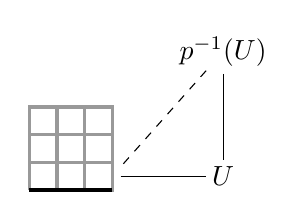
\begin{tikzpicture}[x=1em, y=1em, baseline=1em]
        \draw[very thick, black!40]
            (0,0)--(3,0)--(3,3)--(0,3)--(0,0)
            (1,0)--(1,3) (2,0)--(2,3)
            (0,1)--(3,1) (0,2)--(3,2);
        \draw[very thick] (0,0)--(3,0);
        \draw[-{\tip}, shorten <= 3pt, shorten >= 6pt] (3,.5)--(7,.5);
        \draw[-{\tip}, shorten <= 8pt, shorten >= 6pt] (7,5)--(7,.5);
        \draw[-{\tip}, shorten <= 6pt, shorten >= 8pt, dashed] (3,.5)--(7,5);
        \filldraw 
            (7,0.5) node{$U$}
            (7,5) node{$p^{-1}(U)$};
    \end{tikzpicture}
    \quad\leadsto\quad
    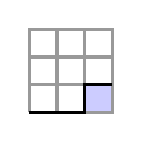
\begin{tikzpicture}[x=1em, y=1em, baseline=1em]
        \fill[blue!20] (2,0)--(2,1)--(3,1)--(3,0);
        \draw[very thick, black!40]
            (0,0)--(3,0)--(3,3)--(0,3)--(0,0)
            (1,0)--(1,3) (2,0)--(2,3)
            (0,1)--(3,1) (0,2)--(3,2);
        \draw[very thick] (0,0)--(2,0)--(2,1)--(3,1);
    \end{tikzpicture}
    \quad\leadsto\cdots\leadsto\quad
    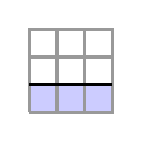
\begin{tikzpicture}[x=1em, y=1em, baseline=1em]
        \fill[blue!20] (0,0)--(0,1)--(3,1)--(3,0);
        \draw[very thick, black!40]
            (0,0)--(3,0)--(3,3)--(0,3)--(0,0)
            (1,0)--(1,3) (2,0)--(2,3)
            (0,1)--(3,1) (0,2)--(3,2);
        \draw[very thick] (0,1)--(3,1);
    \end{tikzpicture}
    \quad\leadsto\cdots\leadsto\quad
    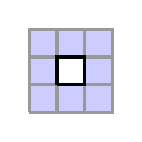
\begin{tikzpicture}[x=1em, y=1em, baseline=1em]
        \fill[blue!20] (0,0)--(0,3)--(3,3)--(3,0);
        \draw[very thick, black!40]
            (0,0)--(3,0)--(3,3)--(0,3)--(0,0)
            (1,0)--(1,3) (2,0)--(2,3)
            (0,1)--(3,1) (0,2)--(3,2);
        \filldraw[very thick, fill=white] (1,1)--(2,1)--(2,2)--(1,2)--(1,1);
    \end{tikzpicture}
    \quad\leadsto \Attention
    \)
\end{center}

We can then extend $H$ iteratively over the smaller cubes "row by row". In every situation this amounts to choosing a solution to the relative lifting problem for a globally trivial fibre bundle.

\end{proof}

\begin{remark}
Not every fibre bundle is a Hurewicz fibration (but actual counter-examples are complicated). A sufficient condition is that the base space be paracompact.
\end{remark}

\begin{remark}

An interesting question: are lifting of homotopies unique? It turns out that they are unique up to homotopy!
\begin{center}
    \begin{tikzcd}[column sep=large]
    X\times\cb{0} \arrow[r] \arrow[d] & E \arrow[d,"p"] \\
    X\times I \arrow[r] \arrow[ur,dashed,"\til H_1", "\til H_2"'] & B
    \end{tikzcd}\qquad
    \begin{tikzcd}
    X\times I\times\cb{0} \cup X\times I\times\cb{1} \arrow[r] \arrow[d] & E \arrow[d,"p"] \\
    X\times I\times I \arrow[r] & B
    \end{tikzcd}
\end{center}\normalmarginpar\todo{I wasn't paying attention, it might be interesting to reconstruct the argument!}

\end{remark}
